\section{Results}\label{sec:results}
% Primary: Thomas & all

\subsection{LANL APEX Simulation Workflows on Celio}

We consider the workload from LANL found in the APEX Workflows
report~\cite{apex} that consists of four simulation applications
classes: EAP, LAP, Silverton and VPIC. The main characteristics of
these classes are reported in Table~\ref{table:lanl}. We simulate the
behavior of these applications over the Celio Platform. \todo{Describe
  Celio here}

\begin{table}
\begin{tabular}{|l|c|c|c|c|}
\hline
 Workflow & EAP & LAP & Silverton & VPIC \\\hline
Workload percentage & 66 & 5.5 & 16.5 & 12 \\\hline
Work time (h) & 262.4 & 64 & 128 & 157.2 \\\hline
Number of cores & 16384 & 4096 & 32768 & 30000 \\\hline
Initial Input (\% of memory) &  3 & 5 & 70 & 10 \\\hline
Final Output (\% of memory) & 105 & 220 & 43 & 270 \\\hline
Checkpoint Size (\% of memory) & 160 & 185 & 350 & 85 \\\hline
\end{tabular}
\caption{LANL Workflow Workload from the APEX Workflows report\label{table:lanl}}
\end{table}

Enough applications are randomly chosen to ensure that the workload
percentage of each class is met within 1\% of its goal, and to gather
a simulated time of at least 2 months (62 days). To serve as the
baseline of comparison, we simulate the execution of each list of
applications without introducing checkpoints, faults, or
interference. In this simulation, we select a segment of the execution
that is 60 days long (to exclude the beginning and end of the
simulation that present uncharacteristic behaviors), and compute 
the resource used by the applications during that time. Since we
consider efficiency from a platform perspective and each application
has a different resource usage, we use the following metric to measure
resource usage: the sum of time each node spends doing a specific
operation. Application usage sums the time spent doing I/O or
computation that was not wasted by a restart due to a failure.

\begin{figure}
  \begin{center}
    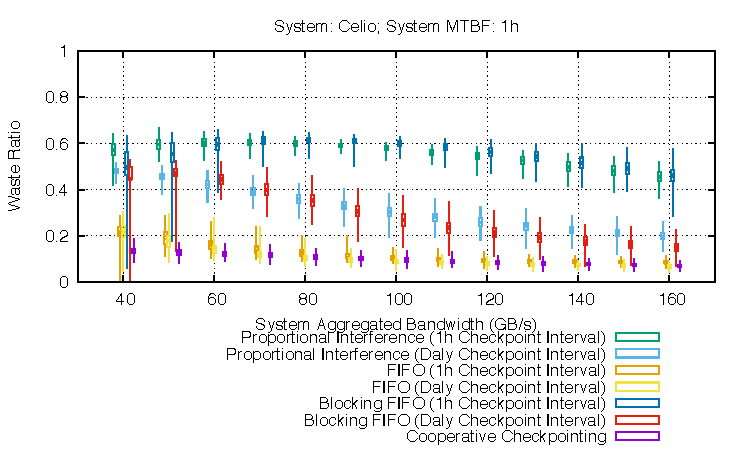
\includegraphics[width=\linewidth]{sim/figures/synthetic-01hMTBF-waste-celio.pdf}
  \end{center}
  \caption{Waste ratio as a function of the system bandwidth for the
    seven I/O and Checkpointing scheduling strategies, and the Celio
    workload \label{fig:celio-1hmtbf}}
\end{figure}

For each checkpointing and I/O scheduling technique presented in
Section~\ref{sec:algorithm}, we then compute the resource waste, as
the sum of application computation or I/O that was wasted due to
failures, and of time checkpointing. We represent below the
performance of each technique by computing the waste ratio, i.e. the
waste resource over a segment of 60 hours divided by the application
usage resource over that same segment for the baseline
simulation. Each simulation is conducted 2,000 times, and the
candelstick extremes represent the first and last decile of the
measures, while the boxes represent the second and third quartile, and
the point in the middle the mean value.

First, we explore the performance of each approach under heavy risks
of failures. Figure~\ref{fig:celio-1hmtbf} represents the waste ratio on Celio,
assuming the MTBF of the system was 1h. We vary the filesystem
bandwidth from 40 GB/s to 160GB/s in order to evaluate the impact of
this parameter. We observe 3 classes of behavior: \propfixed and
\bfifofixed exhibit a waste ratio that remains between 40\% and 60\%
even with a high available bandwidth; \fifodaly, \fifofixed, and
\cooperative increase their performance with the bandwidth, but start
at only 20\% of waste or less (15\% of waste for \cooperative), even
under low filesystem capacity; and \propdaly and \bfifodaly start
at the same level of efficiency as \propfixed and \bfifofixed, and
reach the 20\% of waste as the bandwidth increases. 

This figure shows that with a high frequency of failures, providing
each application with the appropriate checkpoint interval is central
to relieve th filesystem from unecessary (or even detrimental)
checkpoints, but this is not the sole criteria that should be taken
into account. The two strategies that remain with a high waste despite
a high bandwidth rely on a fixed 1h interval. As the figure
illustrates, simply relying on the Daly checkpointing period is not
sufficient to reach the best performance under constrained bandwidth:
at 40GB/s for the filesystem, \propdaly and \bfifodaly experience two
to three times the waste of the other strategies relying on the same
value for the checkpointing period. All strategies that couple the
decision of checkpointing with filesystem availability information
(\fifodaly, \fifofixed, \cooperative) exhibits much better performance
despite low bandwidth. Notably, \cooperative remains the most
efficient technique under all conditions.

\subsection{Prospective Systems}

